\chapter{Analyse et Conception}
\label{chap:Analysis and Design}
\section*{Introduction}

\hspace{\parindent}Cette partie du rapport vise à offrir une vision approfondie et détaillée de l'analyse et de la conception du projet, et à mettre en lumière les choix stratégiques, les décisions clés et les résultats obtenus. Elle constitue une base solide pour la mise en œuvre et le développement futurs du projet. Nous entamons par une analyse fonctionnelle, suivie d'une étude approfondie des besoins, comprenant l'identification des parties prenantes, la collecte des exigences fonctionnelles et la modélisation des processus métier. Ensuite, nous réalisons la conception du système en détaillant l'architecture globale et les différents composants qui le constituent.
\pagebreak







\section{Analyse des besoins}
\subsection{Identification des acteurs}

\hspace{\parindent}Les acteurs, qui représentent des rôles spécifiques joués par les utilisateurs, interagissent avec notre système en tant qu'entités internes ou externes. Ces acteurs peuvent consulter ou modifier l'état du système en envoyant et en recevant des messages contenant des données. Les différents acteurs impliqués dans notre système sont détaillés dans le tableau suivant.


\begin{table}[h]
  \centering
  \captionsetup{justification=centering}
  \begin{tabular}{|p{0.2\textwidth}|p{0.2\textwidth}|p{0.5\textwidth}|}
    \hline
    \textbf{Acteur}       & \textbf{Role}                                & \textbf{Responsabilités}                                                                                                                                                                                                \\ \hline
    \textbf{Super Admin}  & Gestion complète du système                  & Personnel de B3G ayant des privilèges étendus pour gérer les tenants et éditions, les projets (menus et pages), la gestion de contenu (widgets et processus), ainsi que la gestion des utilisateurs et les permissions. \\ \hline
    \textbf{Tenant Admin} & Administration d'un tenant spécifique        & Clients de B3G ayant des privilèges administratifs pour gérer les projets, la gestion de contenu, les utilisateurs et les autorisations au sein de leur propre espace de travail (tenant).                              \\ \hline
    \textbf{End User}     & Consultation des projets/applications créés. & Personne ou entité qui utilise les plateformes créées par un tenant pour accéder aux fonctionnalités, contenus et services proposés.                                                                                    \\ \hline
  \end{tabular}
  \caption{Liste des acteurs}
  \label{tab:actors}
\end{table}

\textbf{NB} : "Tenant" dans ce contexte se réfère à une instance spécifique de l'application, souvent déployée pour un client ou une organisation spécifique. Chaque tenant fonctionne comme une entité indépendante, avec ses propres données, configurations et utilisateurs.

\subsection{Besoins fonctionnels}

\hspace{\parindent} Les besoins fonctionnels décrivent les fonctionnalités et les services essentiels que notre système doit offrir pour satisfaire les attentes des utilisateurs et des parties prenantes. Voici les besoins fonctionnels identifiés pour notre projet :

\begin{itemize}
  \item \textbf{Gestion des utilisateurs :}\\
        Authentification et autorisation, chaque acteur doit obligatoirement s'authentifier avant d'interagir avec le système.Ainsi que le système doit gérer les permissions en fonction des rôles des utilisateurs (Super Admin, Tenant Admin, Utilisateur Final).


        Les Super Admins et les Tenant Admins doivent pouvoir créer, modifier et supprimer des comptes utilisateurs.

  \item \textbf{Gestion des tenants :}\\
        Pour la création et configuration des tenants, Les Super Admins doivent pouvoir créer et configurer de nouveaux tenants. Ainsi que les Tenant Admins doivent pouvoir configurer les paramètres de leur propre tenant, notamment les préférences et les règles spécifiques.

        Quant à la gestion des données et des configurations, chaque tenant doit disposer de ses propres données et configurations isolées des autres tenants pour garantir la sécurité et la confidentialité.

  \item \textbf{Gestion des projets et du contenu :}\\
        Les Tenant Admins doivent pouvoir créer, modifier et supprimer des projets au sein de leur tenant.

        Les projets doivent pouvoir être configurés avec des menus, des pages et des widgets spécifiques selon les besoins du tenant.

        Les Tenant Admins doivent pouvoir ajouter, éditer et supprimer du contenu dans les projets, y compris les widgets et les processus.

        Organisation et structuration du contenu pour une navigation efficace et intuitive pour les utilisateurs finaux.

  \item \textbf{Gestion des autorisations :}\\
        Les Super Admins doivent pouvoir définir des autorisations pour les différents rôles au niveau global.

        Les Tenant Admins doivent pouvoir définir des autorisations spécifiques pour les utilisateurs au sein de leur tenant, en fonction des projets et des contenus.

        Le système doit permettre de contrôler les droits d'accès, de modification et de suppression pour chaque utilisateur ou groupe d'utilisateurs en fonction de leur rôle et des autorisations définies.

  \item \textbf{Gestion des éditions :}\\
        Les Super Admins doivent pouvoir créer et configurer différentes éditions du système, adaptées à des besoins spécifiques ou à des types de clients particuliers.

        Les Super Admins doivent pouvoir personnaliser chaque édition en fonction des besoins des clients, y compris les fonctionnalités disponibles, les thèmes et les configurations spécifiques.

        Les Super Admins doivent pouvoir mettre à jour et maintenir les éditions, incluant l'application de nouvelles fonctionnalités, correctifs et améliorations spécifiques à chaque édition.

\end{itemize}



\subsection{Besoins non fonctionnels}

\hspace{\parindent}Les besoins non fonctionnels définissent les qualités et les contraintes auxquelles le système doit répondre pour garantir sa performance, sa sécurité et sa convivialité. Voici les principaux besoins non fonctionnels identifiés pour notre projet :
\begin{itemize}
  \item \textbf{Sécurité :}
        \begin{enumerate}
          \item Protection des données sensibles et conformité aux normes de sécurité.
          \item Cryptage des données et gestion des vulnérabilités.
        \end{enumerate}

  \item \textbf{Performance :}
        \begin{enumerate}
          \item Temps de réponse rapide et capacité à gérer une charge élevée.
          \item Optimisation des temps de chargement.
        \end{enumerate}

  \item \textbf{Disponibilité :}\\
        Garantir un temps de disponibilité élevé, visant à atteindre un taux cible de disponibilité de 90\%, et mettre en place des mécanismes de récupération pour assurer une continuité de service en cas de défaillance.

  \item \textbf{Facilité d'Utilisation :}
        \begin{enumerate}
          \item Interface utilisateur conviviale et documentation complète.

          \item Formation et support pour les utilisateurs.
        \end{enumerate}

  \item \textbf{Interopérabilité :}\\
        Capacité à intégrer avec d'autres systèmes et à échanger des données.
\end{itemize}






\section{Conception}

\hspace{\parindent}Maintenant que l'analyse a été finalisée, nous sommes prêts à passer à la phase de conception. Cette étape consiste à formaliser les besoins fonctionnels du projet en utilisant des diagrammes UML. Ces diagrammes permettent de représenter le comportement fonctionnel ainsi que la structure du système de manière claire et précise.

\subsection{Diagramme de cas d’utilisation global}

\hspace{\parindent}Le diagramme de cas d'utilisation, un composant essentiel des diagrammes UML de comportement, est utilisé pour illustrer le fonctionnement d'un système et saisir ses exigences. Il expose les fonctionnalités principales du système ainsi que son domaine d'application, tout en mettant en avant les interactions entre le système et les acteurs impliqués. Les cas d'utilisation et les acteurs figurant dans ces diagrammes décrivent les actions réalisées par le système et la manière dont les acteurs interagissent avec celui-ci, sans entrer dans les détails de son fonctionnement interne. Conformément à cette définition, la figure suivante présente le diagramme de cas d'utilisation global du système, mettant en scène trois acteurs : \textbf{le Super Admin, le Tenant Admin} et \textbf{l'Utilisateur final (End user)}.


%\textbf{-------Insert diag cas d'utilisation global---------}


\begin{figure}[H]
  \centering
  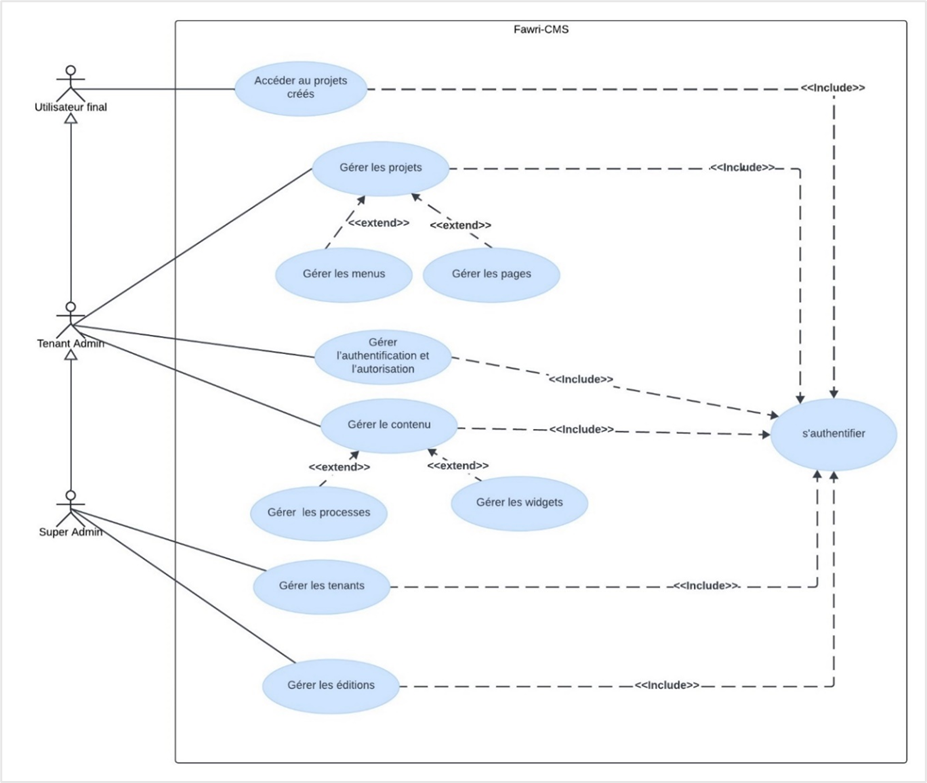
\includegraphics[width=17cm]{Figures/use case globale.png}
  \caption{Diagramme de cas d'utilisation global}
  %\label{fig:my_label} %Optional (If you want to reference the figure in later chapters)
\end{figure}





\subsection{Diagramme de cas d’utilisation : Gestion des projets}

\hspace{\parindent}Ce diagramme détaille les cas d'utilisation pour la gestion des projets, incluant la gestion des pages et des menus. Il précise les fonctionnalités et les cas d'utilisation ainsi que les interactions avec les différents acteurs.

% \textbf{----------Insert diag cas d'utilisation gestion des projets-----------}


\begin{figure}[H]
  \centering
  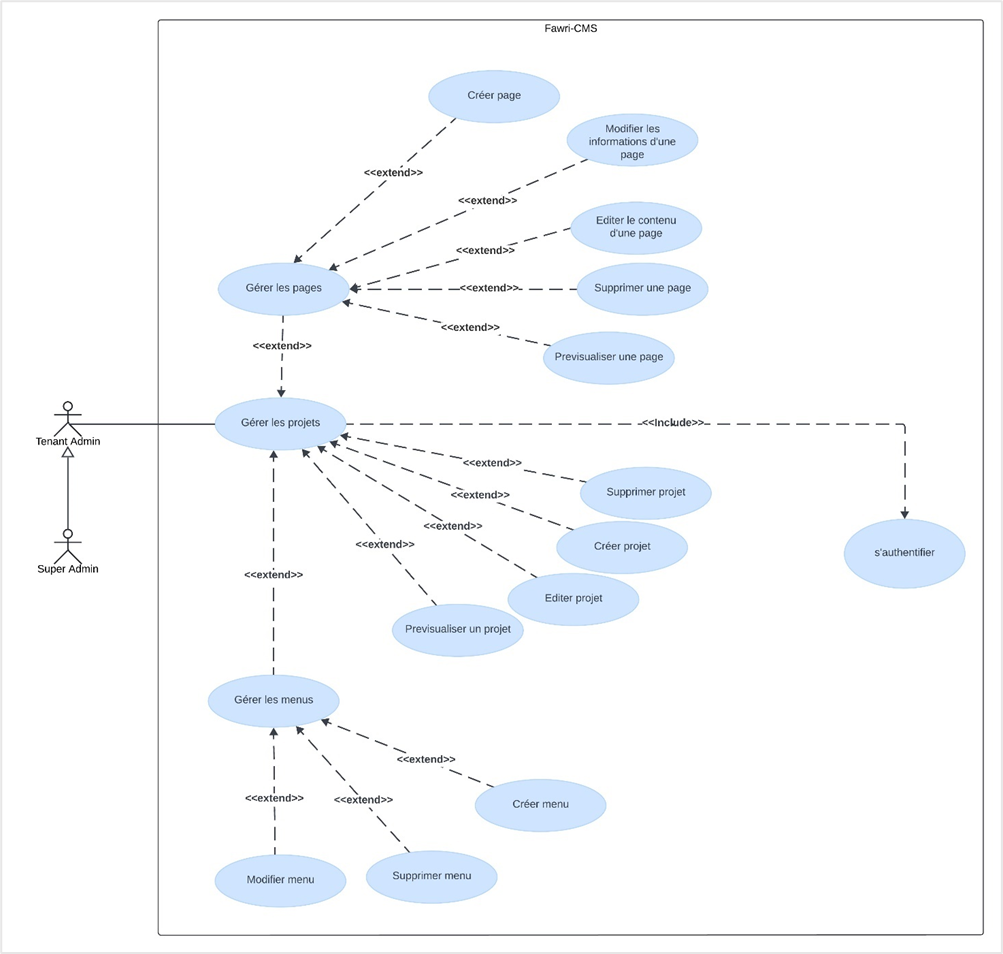
\includegraphics[width=17cm]{Figures/use case gestion des projets.png}
  \caption{Diagramme de cas d'utilisation : gestion des projets}
  %\label{fig:my_label} %Optional (If you want to reference the figure in later chapters)
\end{figure}



\subsection{Diagramme de cas d’utilisation : Gestion de contenu}
\hspace{\parindent}Dans cette partie, nous allons présenter un diagramme de cas d'utilisation qui détaille les différents aspects de la gestion de contenu au sein de notre système Fawri-CMS. Ce diagramme met en lumière les principales fonctionnalités, telles que la gestion des widgets et des processus. Il illustre comment les acteurs, comme les super administrateurs et les administrateurs de tenants, interagissent avec le système pour créer, éditer, supprimer des widgets, et intégrer des processus dans les pages du CMS. Le diagramme suivant représente le diagramme de cas d'utilisation pour la gestion de contenu :

% \textbf{--------Insert diag cas d'utilisation Gestion de contenu--------}

\begin{figure}[H]
  \centering
  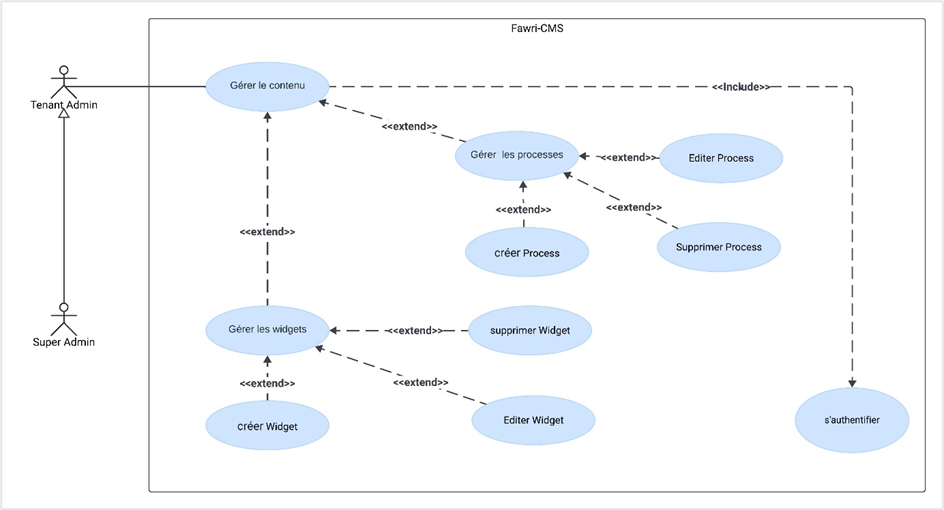
\includegraphics[width=17cm]{Figures/gestion de contenu.png}
  \caption{Diagramme de cas d'utilisation : gestion de contenu}
  %\label{fig:my_label} %Optional (If you want to reference the figure in later chapters)
\end{figure}



\subsection{Diagramme de cas d'utilisation : Gestion des tenants, éditions et permissions}

\hspace{\parindent}Dans cette partie, nous allons présenter un diagramme de cas d'utilisation qui détaille les différents aspects de la gestion des tenants, des éditions et des permissions au sein de notre système Fawri-CMS. Ce diagramme met en lumière les principales fonctionnalités nécessaires à la gestion efficace des tenants, y compris la création, l'édition et la suppression des tenants, ainsi que la gestion des rôles et des permissions associés. Il illustre comment les acteurs, tels que les super administrateurs et les administrateurs de tenants, interagissent avec le système pour administrer ces aspects critiques du CMS.

Le diagramme suivant représente les cas d'utilisation pour la gestion des tenants, l'édition et les permissions dans notre système Fawri-CMS :
% \textbf{-----Insert diag cas d'utilisation Gestion des tenants, éditions et permissions----}

\begin{figure}[H]
  \centering
  \includegraphics[width=17cm]{Figures/Gestion des tenants éditions et permissions .png}
  \caption{Diagramme de cas d'utilisation : gestion des tenants, éditions et permissions}
  %\label{fig:my_label} %Optional (If you want to reference the figure in later chapters)
\end{figure}





\subsection{Diagramme de classes}
\hspace{\parindent}Dans cette partie, nous allons présenter le diagramme de classes de notre système Fawri-CMS. Ce diagramme offre une vue détaillée des classes du système ainsi que leurs relations. Il illustre comment les entités principales interagissent entre elles et comment les différentes fonctionnalités sont implémentées à travers ces interactions.

Le diagramme de classes met en évidence les attributs et les méthodes des classes, fournissant ainsi une vue structurelle de notre application. Il inclut des classes pour la gestion des projets, des pages, des menus, des widgets, des tenants et des permissions, montrant comment ces éléments s'intègrent pour fournir les fonctionnalités complètes du CMS.

Le diagramme suivant représente la structure des classes dans notre système Fawri-CMS

% \textbf{---Insert diag cas de class----}


\begin{figure}[H]
  \centering
  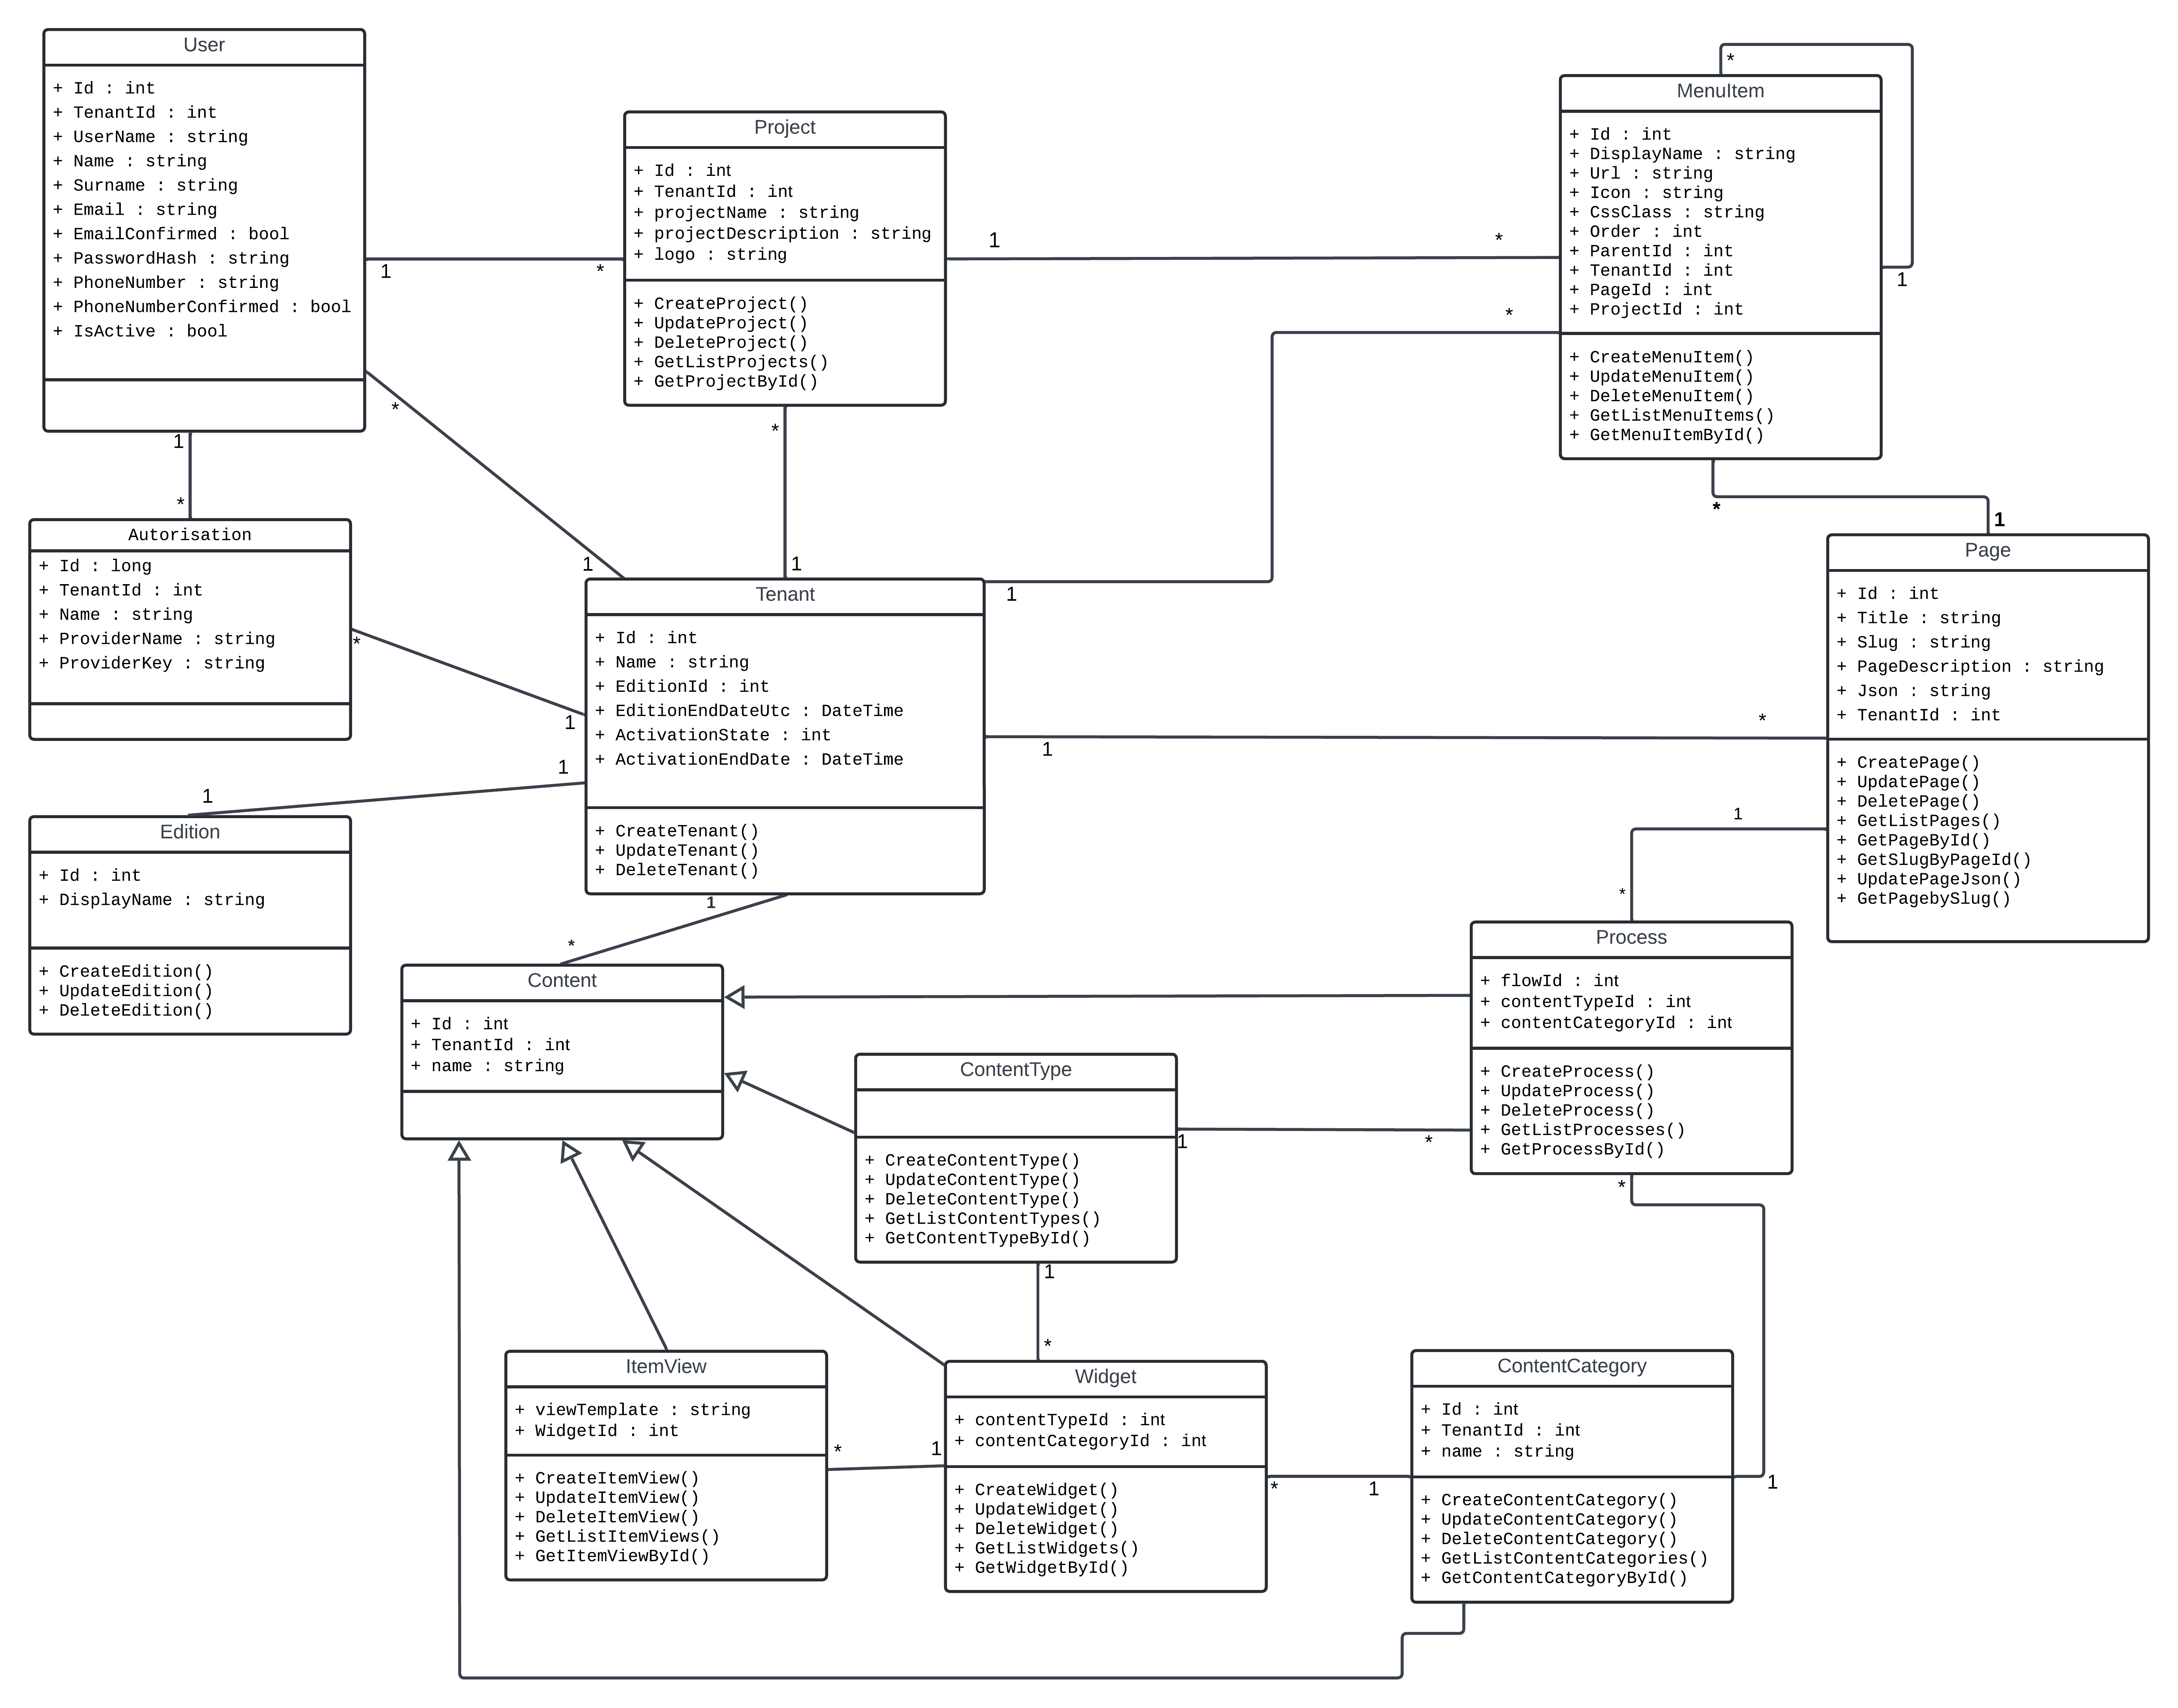
\includegraphics[width=17cm]{Figures/diag de classe.png}
  \caption{Diagramme de classes}
  %\label{fig:my_label} %Optional (If you want to reference the figure in later chapters)
\end{figure}




\textbf{User} : Représente les utilisateurs du système avec des informations générales et des mécanismes d'authentification.

\textbf{Autorisation} : Gère les autorisations et les rôles des utilisateurs dans le système.

\textbf{Project} : Gère les projets créés par les utilisateurs, y compris les opérations de création, mise à jour et suppression.

\textbf{MenuItem} : Représente les éléments de menu associés aux projets, permettant la navigation dans le système.

\textbf{Page} : Gère les pages de contenu au sein des projets, y compris leur création, mise à jour et suppression.

\textbf{Process} : Représente les processus associés aux contenus, gérant leur cycle de vie dans le système.

\textbf{Tenan}t : Gère les tenants, qui sont des instances spécifiques du système déployées pour différents clients ou organisations.

\textbf{Edition} : Gère les éditions du système, qui sont des versions personnalisées adaptées à des besoins spécifiques des clients.

\textbf{Conten} : Gère le contenu au sein des tenants, permettant la création et l'organisation du contenu.

\textbf{ContentTy} : Définit les types de contenu pouvant être créés et gérés dans le système.

\textbf{Widget} : Gère les widgets, qui sont des composants réutilisables dans les pages et projets.

\textbf{ContentCategory} : Organise les contenus en différentes catégories pour une meilleure gestion et structuration.

\textbf{ItemView} : Représente les vues d'éléments, définissant comment les widgets sont affichés dans le système.



\subsection{Diagramme de séquence}


\subsubsection{Diagramme de séquence : Récupération de la liste des processus}

\hspace{\parindent}Le diagramme de séquence ci-dessous illustre le processus par lequel le tenant admin ou le super admin interagit avec Fawri-CMS pour récupérer la liste des processus disponibles depuis l'API Fawri-Flow. Ce diagramme décrit les échanges entre les différents acteurs et systèmes impliqués dans cette opération.
\\
% \textbf{-------insert Diagramme de séquence : Récupération de la liste des processus-------}

\begin{figure}[H]
  \centering
  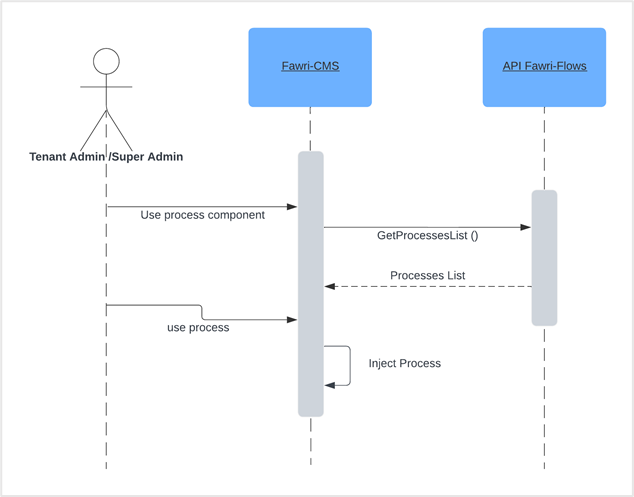
\includegraphics[width=11cm]{Figures/Diagramme_sequence _Recuperation_list_proc.png}
  \caption{Diagramme de séquence  Récupération de la liste des processus}
  %\label{fig:my_label} %Optional (If you want to reference the figure in later chapters)
\end{figure}


\subsubsection{Diagramme de séquence : Gestion des projets}
\hspace{\parindent}Le diagramme de séquence ci-dessous montre le processus de gestion des projets au sein de Fawri-CMS. Il décrit les interactions entre le tenant admin/super admin, Fawri-CMS, et la base de données (DB) lors de la création et de la gestion des projets, les pages associées et les éléments de menu.
\\
\\
\textbf{-------insert Diagramme de séquence : Gestion des projets-------}
\\
\\




\subsubsection{Diagramme de séquence : Gestion des permissions}
\hspace{\parindent}Le diagramme de séquence ci-dessous illustre le processus de gestion des permissions dans Fawri-CMS. Il décrit les interactions entre le super admin/tenant admin, Fawri-CMS, et la base de données (DB) lors de la création de rôles, la gestion des permissions, la définition des autorisations, et l'ajout d'utilisateurs aux rôles.
\\
\\
\textbf{-------insert Diagramme de séquence : Gestion des permissions-------}
\\
\\



\subsubsection{Diagramme de séquence : Gestion des éditions et des tenants}

\hspace{\parindent}Ce diagramme de séquence illustre le processus de gestion des éditions et des tenants dans Fawri-CMS. Il décompose les interactions entre le super administrateur, Fawri-CMS et la base de données (DB) en étapes claires et concises, couvrant les actions de création d'éditions, de gestion des tenants.
\\
\\
\textbf{-------insert Diagramme de séquence : Gestion des éditions et des tenants-------}
\\
\\


\subsubsection{Diagramme d'activité : Gestion des éditions, des tenants et des projets}
\hspace{\parindent}Le diagramme d'activité ci-dessous illustre le processus de gestion des éditions, des tenants et des projets au sein de Fawri-CMS.
\\
\\
\textbf{-------insert Diagramme-------}
\\
\\




\subsubsection{Diagramme d'activité : Gestion des Permissions}
\hspace{\parindent}Le diagramme d'activité ci-dessous illustre le processus de gestion des permissions au sein de Fawri-CMS. Il décrit les étapes et les décisions prises par le super admin/tenant admin pour créer, modifier et gérer les permissions des utilisateurs, des rôles, et les autorisations associées.
\\
\\
\textbf{-------insert Diagramme-------}
\\
\\






\section{Charte Graphique}

\hspace{\parindent}La charte graphique est essentielle pour garantir une identité visuelle cohérente et professionnelle à travers toutes les interfaces et supports du projet Fawri-CMS. Elle définit les règles de présentation visuelle et les standards à respecter pour tous les éléments graphiques de l'application.

\subsection{Logo et Identité Visuelle :}

\hspace{\parindent}Le logo doit être utilisé dans toutes les communications officielles et sur toutes les pages de l'application. Il est crucial pour l'identité de la marque.

\textbf{Format} : SVG ou PNG pour assurer une haute qualité et une adaptabilité.

\textbf{Utilisation} : En-têtes de page, pieds de page, documents marketing et matériel de présentation. Il doit être placé de manière cohérente, généralement en haut à gauche de chaque page.
\\
\begin{figure}[H]
  \centering
  
\includegraphics[width=6cm]{Figures/fawri_cms_logo.PNG}
  \caption{Logo Fawri CMS}
  %\label{fig:my_label} %Optional (If you want to reference the figure in later chapters)
\end{figure}


\subsection{Palette de couleurs}
\hspace{\parindent}Les couleurs jouent un rôle crucial dans l'identité visuelle de Fawri-CMS. Dans notre projet, nous avons utilisé la palette de couleurs suivante :
\\
\begin{figure}[H]
  \centering
  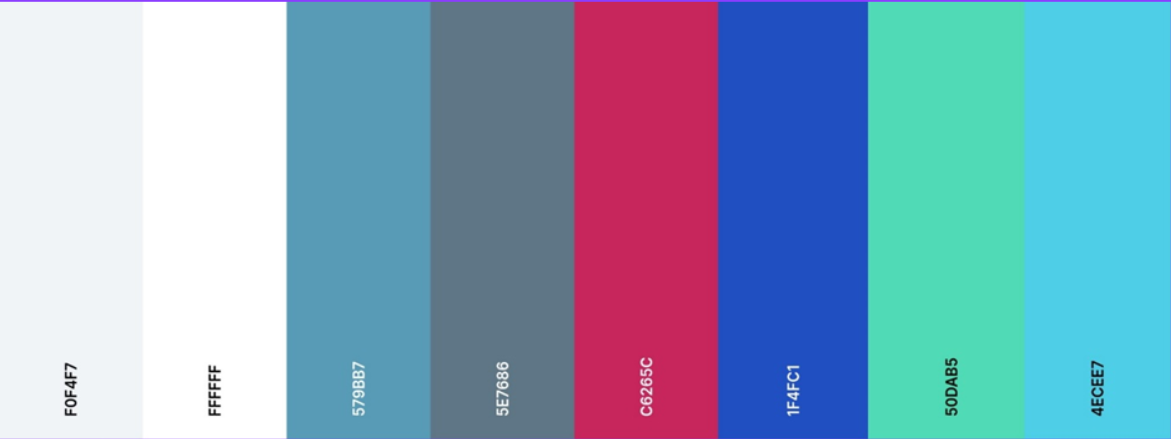
\includegraphics[width=12cm]{Figures/palette.PNG}
  \caption{La palette des couleurs}
  %\label{fig:my_label} %Optional (If you want to reference the figure in later chapters)
\end{figure}



\subsection{Typographie}
\hspace{\parindent}La typographie contribue à la lisibilité et à la cohérence visuelle de l'application Fawri-CMS.

\textbf{Police principale} : Sans-serif

La police principale est principalement utilisée pour les titres et les sous-titres, apportant une distinction claire entre les sections. Elle est également employée dans le corps du texte, les menus, les boutons, ainsi que dans les cellules des tableaux.

\begin{itemize}
  \item Titre 1 (h1) : 20 px

  \item Menu Items : 14 px

  \item Titre des colonnes : 14 px

  \item Contenu des tables : 14 px

  \item Texte du bouton : 14 px
\end{itemize}










\subsection{Boutons et Interactions}
\hspace{\parindent}Dans le cadre de notre projet Fawri-CMS, les boutons et les éléments interactifs doivent être clairement définis et facilement identifiables par les utilisateurs. Une attention particulière est accordée à leur conception pour garantir une expérience utilisateur optimale. Cela inclut l'utilisation de couleurs distinctes, de tailles appropriées et de styles cohérents pour tous les boutons et éléments interactifs afin de s'assurer qu'ils se démarquent visuellement et sont intuitivement reconnaissables pour les utilisateurs finaux.

\textbf{Boutons primaires :}
\begin{itemize}
  \item Couleur de fond : Bleu (\#1F4FC1)

  \item Texte : Blanc (\#FFFFFF)

  \item Bordure : 2px arrondie
\end{itemize}

\textbf{Boutons secondaires :}
\begin{itemize}
  \item Couleur de fond : (\#FFFFFF)

  \item Texte : Shadow Blue (\#5E7686)

  \item Bordure Solide Shadow Blue (\#5E7686)
\end{itemize}

\textbf{Boutons d'alerte}
\begin{itemize}
  \item Couleur de fond : Rouge (\#FF3300)

  \item Texte : Blanc (\#FFFFFF)

  \item Bordure : 2px arrondie
\end{itemize}










\subsection{Icônes}
\hspace{\parindent}Dans ce projet, nous avons utilisé la bibliothèque d'icônes Font Awesome.
\\
\begin{figure}[H]
  \centering
  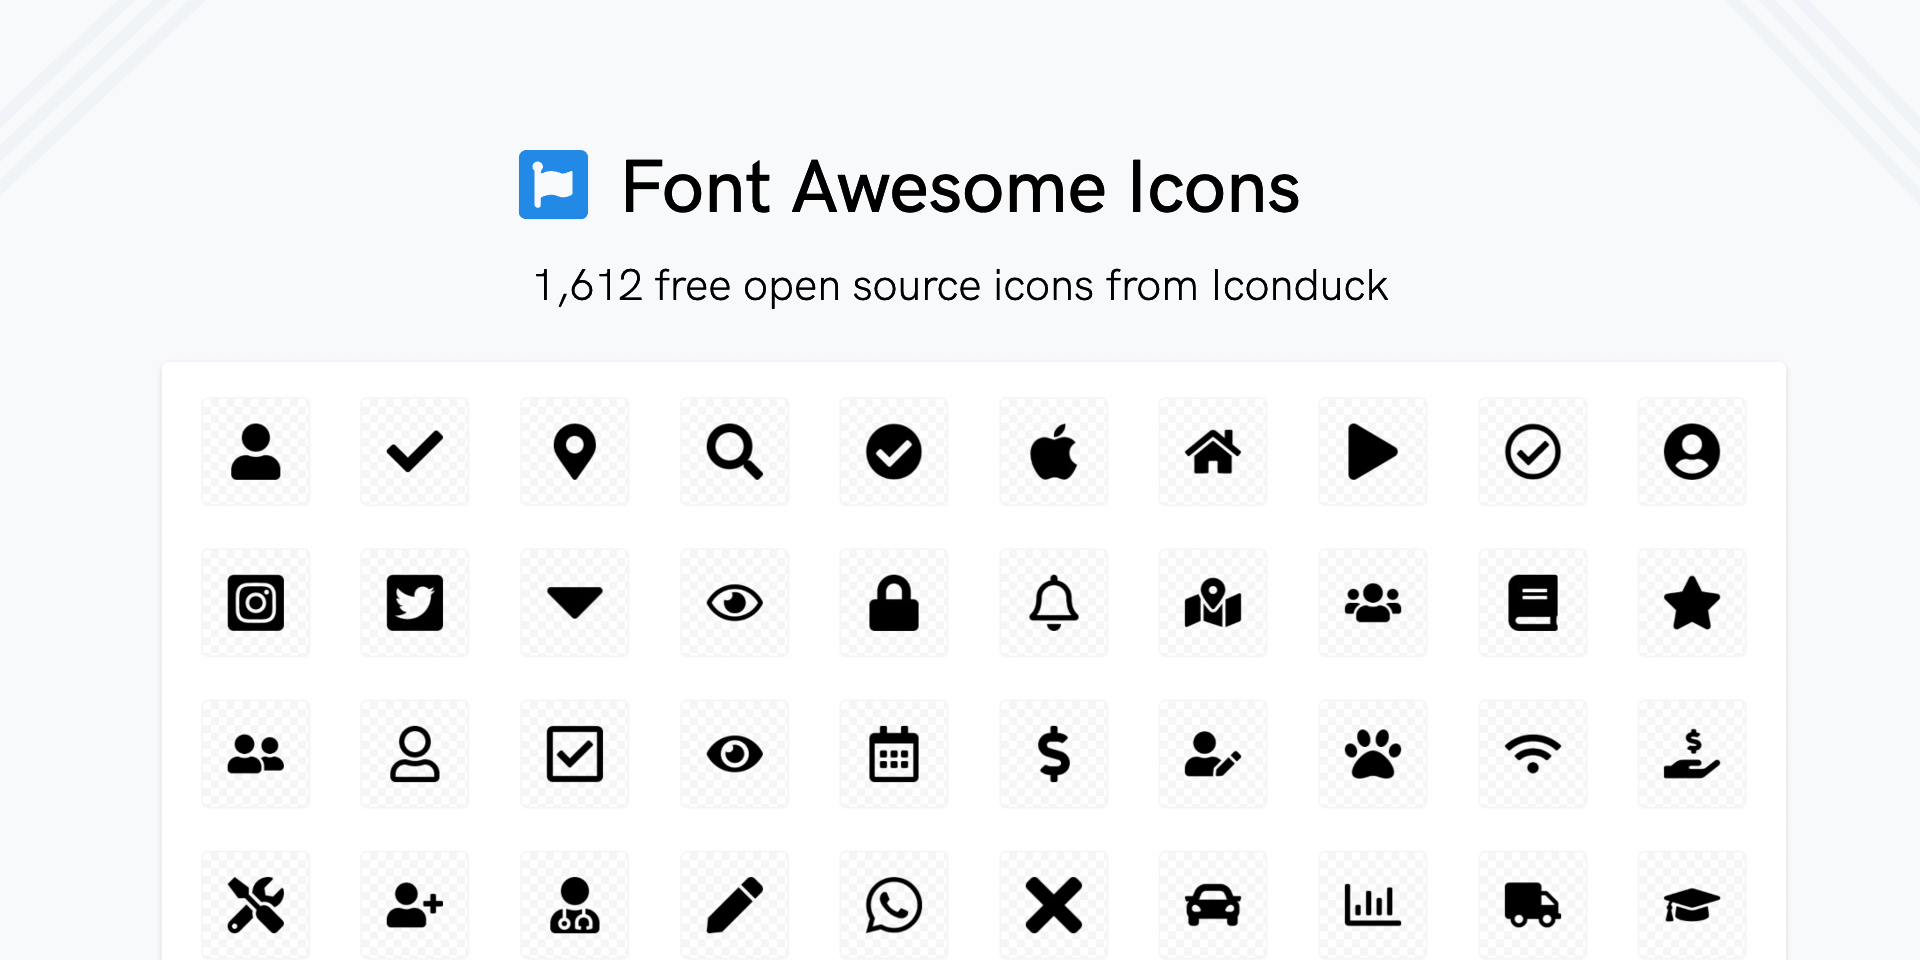
\includegraphics[width=15cm]{Figures/icons.PNG}
  \caption{La bibliothèque d'icons Font Awsome}
  %\label{fig:my_label} %Optional (If you want to reference the figure in later chapters)
\end{figure}











\subsection{La Conception d'Interfaces :}

\hspace{\parindent}Dans notre projet, Figma a joué un rôle central dans la conception des interfaces graphiques de Fawri-CMS. En tant qu'outil principal, il a offert une plateforme collaborative en temps réel ainsi que des fonctionnalités avancées pour créer des prototypes interactifs.

\textbf{Conception d'interfaces utilisateur} : Figma nous a permis de créer des maquettes et des prototypes interactifs pour les différentes interfaces de notre application, y compris les pages d'accueil, les formulaires de saisie de données, etc.

\textbf{Prototypage} : Grâce à ses fonctionnalités de prototypage avancées, nous avons pu simuler les interactions utilisateur et tester les flux de navigation avant le développement. Cela nous a permis d'identifier les problèmes d'expérience utilisateur et d'itérer rapidement sur les designs.
\\
\begin{figure}[H]
  \centering
  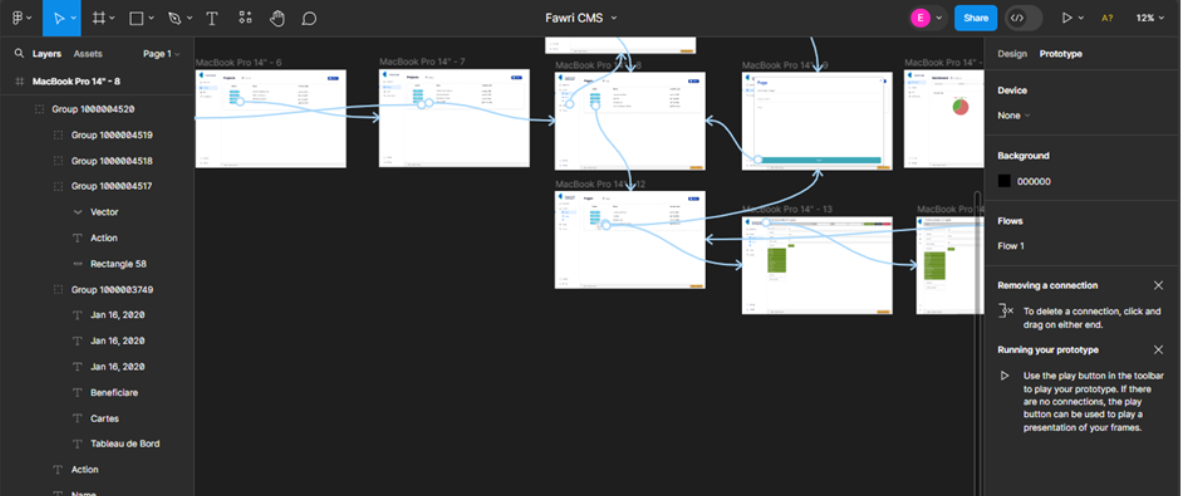
\includegraphics[width=17cm]{Figures/figma.PNG}
  \caption{La maquette d'interactivité de l'interface utilisateur de Fawri CMS}
  %\label{fig:my_label} %Optional (If you want to reference the figure in later chapters)
\end{figure}
















% \begin{longtable}[c]{| m{4.4cm} | m{11cm} |}
% \caption{Long table 1}\\
%  \hline

%  Cell & Description  \\ 
%  \hline
%  \endfirsthead

%  \hline

%  Cell & Description  \\ 
%  \hline
%  \endhead

%         \hline
%           Element11 & Element21 \\
%         \hline
%           Element12 & Element22 \\
%         \hline
%           Element13 & Element23 \\
%         \hline
%           Element14 & Element24 \\
%         \hline
%           Element15 & Element25 \\
%         \hline
%           Element16 & Element26 \\
%         \hline
%           Element17 & Element27 \\
%         \hline
%           Element18 & Element28 \\
%         \hline
%           Element19 & Element29 \\
%         \hline
%           Element110 & Element210 \\
%         \hline
%           Element111 & Element211 \\
%         \hline
%           Element112 & Element212 \\
%         \hline
%           Element113 & Element213 \\
%         \hline
%           Element114 & Element214 \\
%         \hline

%  \end{longtable}




\newpage

\section*{Conclusion}


\hspace{\parindent}Le chapitre d'Analyse et Conception a été une étape cruciale dans la planification de notre projet. En analysant les besoins, nous avons identifié les acteurs clés et détaillé les fonctionnalités du système, couvrant la gestion des utilisateurs, des tenants, des projets, du contenu et des autorisations. Dans la phase de Conception, nous avons élaborer des diagrammes pour illustrer l'architecture globale du système, ainsi qu'une charte graphique définissant l'identité visuelle du projet. Ces éléments fournissent une base solide pour le développement ultérieur, en assurant une compréhension claire des besoins des utilisateurs, une conception architecturale cohérente et une direction visuelle pour l'interface utilisateur.


























